%Packages are included below, these are akin to libraries in other programming languages. As far as I can tell, there is no reason to reduce the number of packages included in a document. It might compile faster, but overleaf compiles fast so this should not be an issue.
\documentclass[
fontsize=11pt,
paper=a4,
abstract=true,
headings=standardclasses,
chapterprefix=false,
numbers=noenddot,
parskip=half+, % comment this out if you do not want an empty half line between paragraphs, but please read the KomaScript Guide and search for parskip (around page 82): ftp://ftp.dante.de/pub/tex/macros/latex/contrib/koma-script/scrguide.pdf
]{scrreprt}
% \documentclass[11pt]{report} %tells the compiler that this is a 'report' style document, and the main font size.
\usepackage{setspace} %allows the use of '\doublespace' to set line spacing
\usepackage[utf8]{inputenc} %inclusion of this is optional, overleaf includes it in its compiler so it is not necessary, it may be necessary for other compilers.
\usepackage{wrapfig} %if it is desirable to wrap text (see https://www.overleaf.com/learn/latex/Wrapping_text_around_figures).
\usepackage{graphicx} %this allows graphics to be put in easily
\usepackage{float}%this allows you to put them in good places
\usepackage[version=4]{mhchem} %this is good for chemical reactions
\usepackage{amsmath} %maths package
\usepackage{amssymb} %symbol package
\usepackage{textcomp,gensymb} %more symbols (eg \degree)
\usepackage{appendix} %self explanatory
\usepackage{colortbl} %good for colouring in cells on a table
\usepackage{rotating} %allows you to rotate graphics
\usepackage{bm} %helps bold things
\usepackage{multirow} %for tables
\usepackage{longtable} %for long tables
\usepackage{booktabs} %more tables
\usepackage{caption} %allows captions for graphics
\usepackage[nottoc]{tocbibind} %adds the bibliography to the table of contents
\usepackage{subcaption} %allows subcaption for multiple images in one graphic

\PassOptionsToPackage{hyphens}{url}\usepackage{hyperref}
\usepackage{hyperref} %this is great for putting hyperreferences in the document.
\usepackage[table]{xcolor} %more colouring of tables
\definecolor{Gray}{gray}{0.9} %this defines a colour to be used and gives it a name. This is a colour called 'Gray' it is 'gray' with transparency 0.9
%  %%%%%%%%%%%%%%%%%%%%%%%%%%%%%%%%%%%%%%%%%%%%%%%%%%%%%%%%%%%%%%%%%%%%%%%%%%%%%%%% 
%%% ~ Arduino Language - Arduino IDE Colors ~                                  %%%
%%%                                                                            %%%
%%% Kyle Rocha-Brownell | 10/2/2017 | No Licence                               %%%
%%% -------------------------------------------------------------------------- %%%
%%%                                                                            %%%
%%% Place this file in your working directory (next to the latex file you're   %%%
%%% working on).  To add it to your project, place:                            %%%
%%%     %%%%%%%%%%%%%%%%%%%%%%%%%%%%%%%%%%%%%%%%%%%%%%%%%%%%%%%%%%%%%%%%%%%%%%%%%%%%%%%% 
%%% ~ Arduino Language - Arduino IDE Colors ~                                  %%%
%%%                                                                            %%%
%%% Kyle Rocha-Brownell | 10/2/2017 | No Licence                               %%%
%%% -------------------------------------------------------------------------- %%%
%%%                                                                            %%%
%%% Place this file in your working directory (next to the latex file you're   %%%
%%% working on).  To add it to your project, place:                            %%%
%%%     %%%%%%%%%%%%%%%%%%%%%%%%%%%%%%%%%%%%%%%%%%%%%%%%%%%%%%%%%%%%%%%%%%%%%%%%%%%%%%%% 
%%% ~ Arduino Language - Arduino IDE Colors ~                                  %%%
%%%                                                                            %%%
%%% Kyle Rocha-Brownell | 10/2/2017 | No Licence                               %%%
%%% -------------------------------------------------------------------------- %%%
%%%                                                                            %%%
%%% Place this file in your working directory (next to the latex file you're   %%%
%%% working on).  To add it to your project, place:                            %%%
%%%    \input{arduinoLanguage.tex}                                             %%%
%%% somewhere before \begin{document} in your latex file.                      %%%
%%%                                                                            %%%
%%% In your document, place your arduino code between:                         %%%
%%%   \begin{lstlisting}[language=Arduino]                                     %%%
%%% and:                                                                       %%%
%%%   \end{lstlisting}                                                         %%%
%%%                                                                            %%%
%%% Or create your own style to add non-built-in functions and variables.      %%%
%%%                                                                            %%%
 %%%%%%%%%%%%%%%%%%%%%%%%%%%%%%%%%%%%%%%%%%%%%%%%%%%%%%%%%%%%%%%%%%%%%%%%%%%%%%%% 


\usepackage{listings}    
\usepackage{courier}

%%% Define Custom IDE Colors %%%
\definecolor{arduinoGreen}    {rgb} {0.17, 0.43, 0.01}
\definecolor{arduinoGrey}     {rgb} {0.47, 0.47, 0.33}
\definecolor{arduinoOrange}   {rgb} {0.8 , 0.4 , 0   }
\definecolor{arduinoBlue}     {rgb} {0.01, 0.61, 0.98}
\definecolor{arduinoDarkBlue} {rgb} {0.0 , 0.2 , 0.5 }

%%% Define Arduino Language %%%
\lstdefinelanguage{Arduino}{
  language=C++, % begin with default C++ settings 
%
%
  %%% Keyword Color Group 1 %%%  (called KEYWORD3 by arduino)
  keywordstyle=\color{arduinoGreen},   
  deletekeywords={  % remove all arduino keywords that might be in c++
                break, case, override, final, continue, default, do, else, for, 
                if, return, goto, switch, throw, try, while, setup, loop, export, 
                not, or, and, xor, include, define, elif, else, error, if, ifdef, 
                ifndef, pragma, warning,
                HIGH, LOW, INPUT, INPUT_PULLUP, OUTPUT, DEC, BIN, HEX, OCT, PI, 
                HALF_PI, TWO_PI, LSBFIRST, MSBFIRST, CHANGE, FALLING, RISING, 
                DEFAULT, EXTERNAL, INTERNAL, INTERNAL1V1, INTERNAL2V56, LED_BUILTIN, 
                LED_BUILTIN_RX, LED_BUILTIN_TX, DIGITAL_MESSAGE, FIRMATA_STRING, 
                ANALOG_MESSAGE, REPORT_DIGITAL, REPORT_ANALOG, SET_PIN_MODE, 
                SYSTEM_RESET, SYSEX_START, auto, int8_t, int16_t, int32_t, int64_t, 
                uint8_t, uint16_t, uint32_t, uint64_t, char16_t, char32_t, operator, 
                enum, delete, bool, boolean, byte, char, const, false, float, double, 
                null, NULL, int, long, new, private, protected, public, short, 
                signed, static, volatile, String, void, true, unsigned, word, array, 
                sizeof, dynamic_cast, typedef, const_cast, struct, static_cast, union, 
                friend, extern, class, reinterpret_cast, register, explicit, inline, 
                _Bool, complex, _Complex, _Imaginary, atomic_bool, atomic_char, 
                atomic_schar, atomic_uchar, atomic_short, atomic_ushort, atomic_int, 
                atomic_uint, atomic_long, atomic_ulong, atomic_llong, atomic_ullong, 
                virtual, PROGMEM,
                Serial, Serial1, Serial2, Serial3, SerialUSB, Keyboard, Mouse,
                abs, acos, asin, atan, atan2, ceil, constrain, cos, degrees, exp, 
                floor, log, map, max, min, radians, random, randomSeed, round, sin, 
                sq, sqrt, tan, pow, bitRead, bitWrite, bitSet, bitClear, bit, 
                highByte, lowByte, analogReference, analogRead, 
                analogReadResolution, analogWrite, analogWriteResolution, 
                attachInterrupt, detachInterrupt, digitalPinToInterrupt, delay, 
                delayMicroseconds, digitalWrite, digitalRead, interrupts, millis, 
                micros, noInterrupts, noTone, pinMode, pulseIn, pulseInLong, shiftIn, 
                shiftOut, tone, yield, Stream, begin, end, peek, read, print, 
                println, available, availableForWrite, flush, setTimeout, find, 
                findUntil, parseInt, parseFloat, readBytes, readBytesUntil, readString, 
                readStringUntil, trim, toUpperCase, toLowerCase, charAt, compareTo, 
                concat, endsWith, startsWith, equals, equalsIgnoreCase, getBytes, 
                indexOf, lastIndexOf, length, replace, setCharAt, substring, 
                toCharArray, toInt, press, release, releaseAll, accept, click, move, 
                isPressed, isAlphaNumeric, isAlpha, isAscii, isWhitespace, isControl, 
                isDigit, isGraph, isLowerCase, isPrintable, isPunct, isSpace, 
                isUpperCase, isHexadecimalDigit, 
                }, 
  morekeywords={   % add arduino structures to group 1
                break, case, override, final, continue, default, do, else, for, 
                if, return, goto, switch, throw, try, while, setup, loop, export, 
                not, or, and, xor, include, define, elif, else, error, if, ifdef, 
                ifndef, pragma, warning,
                }, 
% 
%
  %%% Keyword Color Group 2 %%%  (called LITERAL1 by arduino)
  keywordstyle=[2]\color{arduinoBlue},   
  keywords=[2]{   % add variables and dataTypes as 2nd group  
                HIGH, LOW, INPUT, INPUT_PULLUP, OUTPUT, DEC, BIN, HEX, OCT, PI, 
                HALF_PI, TWO_PI, LSBFIRST, MSBFIRST, CHANGE, FALLING, RISING, 
                DEFAULT, EXTERNAL, INTERNAL, INTERNAL1V1, INTERNAL2V56, LED_BUILTIN, 
                LED_BUILTIN_RX, LED_BUILTIN_TX, DIGITAL_MESSAGE, FIRMATA_STRING, 
                ANALOG_MESSAGE, REPORT_DIGITAL, REPORT_ANALOG, SET_PIN_MODE, 
                SYSTEM_RESET, SYSEX_START, auto, int8_t, int16_t, int32_t, int64_t, 
                uint8_t, uint16_t, uint32_t, uint64_t, char16_t, char32_t, operator, 
                enum, delete, bool, boolean, byte, char, const, false, float, double, 
                null, NULL, int, long, new, private, protected, public, short, 
                signed, static, volatile, String, void, true, unsigned, word, array, 
                sizeof, dynamic_cast, typedef, const_cast, struct, static_cast, union, 
                friend, extern, class, reinterpret_cast, register, explicit, inline, 
                _Bool, complex, _Complex, _Imaginary, atomic_bool, atomic_char, 
                atomic_schar, atomic_uchar, atomic_short, atomic_ushort, atomic_int, 
                atomic_uint, atomic_long, atomic_ulong, atomic_llong, atomic_ullong, 
                virtual, PROGMEM,
                },  
% 
%
  %%% Keyword Color Group 3 %%%  (called KEYWORD1 by arduino)
  keywordstyle=[3]\bfseries\color{arduinoOrange},
  keywords=[3]{  % add built-in functions as a 3rd group
                Serial, Serial1, Serial2, Serial3, SerialUSB, Keyboard, Mouse,
                },      
%
%
  %%% Keyword Color Group 4 %%%  (called KEYWORD2 by arduino)
  keywordstyle=[4]\color{arduinoOrange},
  keywords=[4]{  % add more built-in functions as a 4th group
                abs, acos, asin, atan, atan2, ceil, constrain, cos, degrees, exp, 
                floor, log, map, max, min, radians, random, randomSeed, round, sin, 
                sq, sqrt, tan, pow, bitRead, bitWrite, bitSet, bitClear, bit, 
                highByte, lowByte, analogReference, analogRead, 
                analogReadResolution, analogWrite, analogWriteResolution, 
                attachInterrupt, detachInterrupt, digitalPinToInterrupt, delay, 
                delayMicroseconds, digitalWrite, digitalRead, interrupts, millis, 
                micros, noInterrupts, noTone, pinMode, pulseIn, pulseInLong, shiftIn, 
                shiftOut, tone, yield, Stream, begin, end, peek, read, print, 
                println, available, availableForWrite, flush, setTimeout, find, 
                findUntil, parseInt, parseFloat, readBytes, readBytesUntil, readString, 
                readStringUntil, trim, toUpperCase, toLowerCase, charAt, compareTo, 
                concat, endsWith, startsWith, equals, equalsIgnoreCase, getBytes, 
                indexOf, lastIndexOf, length, replace, setCharAt, substring, 
                toCharArray, toInt, press, release, releaseAll, accept, click, move, 
                isPressed, isAlphaNumeric, isAlpha, isAscii, isWhitespace, isControl, 
                isDigit, isGraph, isLowerCase, isPrintable, isPunct, isSpace, 
                isUpperCase, isHexadecimalDigit, 
                },      
%
%
  %%% Set Other Colors %%%
  stringstyle=\color{arduinoDarkBlue},    
  commentstyle=\color{arduinoGrey},    
%          
%   
  %%%% Line Numbering %%%%
   numbers=left,                    
  numbersep=5pt,                   
  numberstyle=\color{arduinoGrey},    
  %stepnumber=2,                      % show every 2 line numbers
%
%
  %%%% Code Box Style %%%%
  breaklines=true,                    % wordwrapping
  tabsize=2,         
  basicstyle=\ttfamily  
}                                             %%%
%%% somewhere before \begin{document} in your latex file.                      %%%
%%%                                                                            %%%
%%% In your document, place your arduino code between:                         %%%
%%%   \begin{lstlisting}[language=Arduino]                                     %%%
%%% and:                                                                       %%%
%%%   \end{lstlisting}                                                         %%%
%%%                                                                            %%%
%%% Or create your own style to add non-built-in functions and variables.      %%%
%%%                                                                            %%%
 %%%%%%%%%%%%%%%%%%%%%%%%%%%%%%%%%%%%%%%%%%%%%%%%%%%%%%%%%%%%%%%%%%%%%%%%%%%%%%%% 


\usepackage{listings}    
\usepackage{courier}

%%% Define Custom IDE Colors %%%
\definecolor{arduinoGreen}    {rgb} {0.17, 0.43, 0.01}
\definecolor{arduinoGrey}     {rgb} {0.47, 0.47, 0.33}
\definecolor{arduinoOrange}   {rgb} {0.8 , 0.4 , 0   }
\definecolor{arduinoBlue}     {rgb} {0.01, 0.61, 0.98}
\definecolor{arduinoDarkBlue} {rgb} {0.0 , 0.2 , 0.5 }

%%% Define Arduino Language %%%
\lstdefinelanguage{Arduino}{
  language=C++, % begin with default C++ settings 
%
%
  %%% Keyword Color Group 1 %%%  (called KEYWORD3 by arduino)
  keywordstyle=\color{arduinoGreen},   
  deletekeywords={  % remove all arduino keywords that might be in c++
                break, case, override, final, continue, default, do, else, for, 
                if, return, goto, switch, throw, try, while, setup, loop, export, 
                not, or, and, xor, include, define, elif, else, error, if, ifdef, 
                ifndef, pragma, warning,
                HIGH, LOW, INPUT, INPUT_PULLUP, OUTPUT, DEC, BIN, HEX, OCT, PI, 
                HALF_PI, TWO_PI, LSBFIRST, MSBFIRST, CHANGE, FALLING, RISING, 
                DEFAULT, EXTERNAL, INTERNAL, INTERNAL1V1, INTERNAL2V56, LED_BUILTIN, 
                LED_BUILTIN_RX, LED_BUILTIN_TX, DIGITAL_MESSAGE, FIRMATA_STRING, 
                ANALOG_MESSAGE, REPORT_DIGITAL, REPORT_ANALOG, SET_PIN_MODE, 
                SYSTEM_RESET, SYSEX_START, auto, int8_t, int16_t, int32_t, int64_t, 
                uint8_t, uint16_t, uint32_t, uint64_t, char16_t, char32_t, operator, 
                enum, delete, bool, boolean, byte, char, const, false, float, double, 
                null, NULL, int, long, new, private, protected, public, short, 
                signed, static, volatile, String, void, true, unsigned, word, array, 
                sizeof, dynamic_cast, typedef, const_cast, struct, static_cast, union, 
                friend, extern, class, reinterpret_cast, register, explicit, inline, 
                _Bool, complex, _Complex, _Imaginary, atomic_bool, atomic_char, 
                atomic_schar, atomic_uchar, atomic_short, atomic_ushort, atomic_int, 
                atomic_uint, atomic_long, atomic_ulong, atomic_llong, atomic_ullong, 
                virtual, PROGMEM,
                Serial, Serial1, Serial2, Serial3, SerialUSB, Keyboard, Mouse,
                abs, acos, asin, atan, atan2, ceil, constrain, cos, degrees, exp, 
                floor, log, map, max, min, radians, random, randomSeed, round, sin, 
                sq, sqrt, tan, pow, bitRead, bitWrite, bitSet, bitClear, bit, 
                highByte, lowByte, analogReference, analogRead, 
                analogReadResolution, analogWrite, analogWriteResolution, 
                attachInterrupt, detachInterrupt, digitalPinToInterrupt, delay, 
                delayMicroseconds, digitalWrite, digitalRead, interrupts, millis, 
                micros, noInterrupts, noTone, pinMode, pulseIn, pulseInLong, shiftIn, 
                shiftOut, tone, yield, Stream, begin, end, peek, read, print, 
                println, available, availableForWrite, flush, setTimeout, find, 
                findUntil, parseInt, parseFloat, readBytes, readBytesUntil, readString, 
                readStringUntil, trim, toUpperCase, toLowerCase, charAt, compareTo, 
                concat, endsWith, startsWith, equals, equalsIgnoreCase, getBytes, 
                indexOf, lastIndexOf, length, replace, setCharAt, substring, 
                toCharArray, toInt, press, release, releaseAll, accept, click, move, 
                isPressed, isAlphaNumeric, isAlpha, isAscii, isWhitespace, isControl, 
                isDigit, isGraph, isLowerCase, isPrintable, isPunct, isSpace, 
                isUpperCase, isHexadecimalDigit, 
                }, 
  morekeywords={   % add arduino structures to group 1
                break, case, override, final, continue, default, do, else, for, 
                if, return, goto, switch, throw, try, while, setup, loop, export, 
                not, or, and, xor, include, define, elif, else, error, if, ifdef, 
                ifndef, pragma, warning,
                }, 
% 
%
  %%% Keyword Color Group 2 %%%  (called LITERAL1 by arduino)
  keywordstyle=[2]\color{arduinoBlue},   
  keywords=[2]{   % add variables and dataTypes as 2nd group  
                HIGH, LOW, INPUT, INPUT_PULLUP, OUTPUT, DEC, BIN, HEX, OCT, PI, 
                HALF_PI, TWO_PI, LSBFIRST, MSBFIRST, CHANGE, FALLING, RISING, 
                DEFAULT, EXTERNAL, INTERNAL, INTERNAL1V1, INTERNAL2V56, LED_BUILTIN, 
                LED_BUILTIN_RX, LED_BUILTIN_TX, DIGITAL_MESSAGE, FIRMATA_STRING, 
                ANALOG_MESSAGE, REPORT_DIGITAL, REPORT_ANALOG, SET_PIN_MODE, 
                SYSTEM_RESET, SYSEX_START, auto, int8_t, int16_t, int32_t, int64_t, 
                uint8_t, uint16_t, uint32_t, uint64_t, char16_t, char32_t, operator, 
                enum, delete, bool, boolean, byte, char, const, false, float, double, 
                null, NULL, int, long, new, private, protected, public, short, 
                signed, static, volatile, String, void, true, unsigned, word, array, 
                sizeof, dynamic_cast, typedef, const_cast, struct, static_cast, union, 
                friend, extern, class, reinterpret_cast, register, explicit, inline, 
                _Bool, complex, _Complex, _Imaginary, atomic_bool, atomic_char, 
                atomic_schar, atomic_uchar, atomic_short, atomic_ushort, atomic_int, 
                atomic_uint, atomic_long, atomic_ulong, atomic_llong, atomic_ullong, 
                virtual, PROGMEM,
                },  
% 
%
  %%% Keyword Color Group 3 %%%  (called KEYWORD1 by arduino)
  keywordstyle=[3]\bfseries\color{arduinoOrange},
  keywords=[3]{  % add built-in functions as a 3rd group
                Serial, Serial1, Serial2, Serial3, SerialUSB, Keyboard, Mouse,
                },      
%
%
  %%% Keyword Color Group 4 %%%  (called KEYWORD2 by arduino)
  keywordstyle=[4]\color{arduinoOrange},
  keywords=[4]{  % add more built-in functions as a 4th group
                abs, acos, asin, atan, atan2, ceil, constrain, cos, degrees, exp, 
                floor, log, map, max, min, radians, random, randomSeed, round, sin, 
                sq, sqrt, tan, pow, bitRead, bitWrite, bitSet, bitClear, bit, 
                highByte, lowByte, analogReference, analogRead, 
                analogReadResolution, analogWrite, analogWriteResolution, 
                attachInterrupt, detachInterrupt, digitalPinToInterrupt, delay, 
                delayMicroseconds, digitalWrite, digitalRead, interrupts, millis, 
                micros, noInterrupts, noTone, pinMode, pulseIn, pulseInLong, shiftIn, 
                shiftOut, tone, yield, Stream, begin, end, peek, read, print, 
                println, available, availableForWrite, flush, setTimeout, find, 
                findUntil, parseInt, parseFloat, readBytes, readBytesUntil, readString, 
                readStringUntil, trim, toUpperCase, toLowerCase, charAt, compareTo, 
                concat, endsWith, startsWith, equals, equalsIgnoreCase, getBytes, 
                indexOf, lastIndexOf, length, replace, setCharAt, substring, 
                toCharArray, toInt, press, release, releaseAll, accept, click, move, 
                isPressed, isAlphaNumeric, isAlpha, isAscii, isWhitespace, isControl, 
                isDigit, isGraph, isLowerCase, isPrintable, isPunct, isSpace, 
                isUpperCase, isHexadecimalDigit, 
                },      
%
%
  %%% Set Other Colors %%%
  stringstyle=\color{arduinoDarkBlue},    
  commentstyle=\color{arduinoGrey},    
%          
%   
  %%%% Line Numbering %%%%
   numbers=left,                    
  numbersep=5pt,                   
  numberstyle=\color{arduinoGrey},    
  %stepnumber=2,                      % show every 2 line numbers
%
%
  %%%% Code Box Style %%%%
  breaklines=true,                    % wordwrapping
  tabsize=2,         
  basicstyle=\ttfamily  
}                                             %%%
%%% somewhere before \begin{document} in your latex file.                      %%%
%%%                                                                            %%%
%%% In your document, place your arduino code between:                         %%%
%%%   \begin{lstlisting}[language=Arduino]                                     %%%
%%% and:                                                                       %%%
%%%   \end{lstlisting}                                                         %%%
%%%                                                                            %%%
%%% Or create your own style to add non-built-in functions and variables.      %%%
%%%                                                                            %%%
 %%%%%%%%%%%%%%%%%%%%%%%%%%%%%%%%%%%%%%%%%%%%%%%%%%%%%%%%%%%%%%%%%%%%%%%%%%%%%%%% 


\usepackage{listings}    
\usepackage{courier}

%%% Define Custom IDE Colors %%%
\definecolor{arduinoGreen}    {rgb} {0.17, 0.43, 0.01}
\definecolor{arduinoGrey}     {rgb} {0.47, 0.47, 0.33}
\definecolor{arduinoOrange}   {rgb} {0.8 , 0.4 , 0   }
\definecolor{arduinoBlue}     {rgb} {0.01, 0.61, 0.98}
\definecolor{arduinoDarkBlue} {rgb} {0.0 , 0.2 , 0.5 }

%%% Define Arduino Language %%%
\lstdefinelanguage{Arduino}{
  language=C++, % begin with default C++ settings 
%
%
  %%% Keyword Color Group 1 %%%  (called KEYWORD3 by arduino)
  keywordstyle=\color{arduinoGreen},   
  deletekeywords={  % remove all arduino keywords that might be in c++
                break, case, override, final, continue, default, do, else, for, 
                if, return, goto, switch, throw, try, while, setup, loop, export, 
                not, or, and, xor, include, define, elif, else, error, if, ifdef, 
                ifndef, pragma, warning,
                HIGH, LOW, INPUT, INPUT_PULLUP, OUTPUT, DEC, BIN, HEX, OCT, PI, 
                HALF_PI, TWO_PI, LSBFIRST, MSBFIRST, CHANGE, FALLING, RISING, 
                DEFAULT, EXTERNAL, INTERNAL, INTERNAL1V1, INTERNAL2V56, LED_BUILTIN, 
                LED_BUILTIN_RX, LED_BUILTIN_TX, DIGITAL_MESSAGE, FIRMATA_STRING, 
                ANALOG_MESSAGE, REPORT_DIGITAL, REPORT_ANALOG, SET_PIN_MODE, 
                SYSTEM_RESET, SYSEX_START, auto, int8_t, int16_t, int32_t, int64_t, 
                uint8_t, uint16_t, uint32_t, uint64_t, char16_t, char32_t, operator, 
                enum, delete, bool, boolean, byte, char, const, false, float, double, 
                null, NULL, int, long, new, private, protected, public, short, 
                signed, static, volatile, String, void, true, unsigned, word, array, 
                sizeof, dynamic_cast, typedef, const_cast, struct, static_cast, union, 
                friend, extern, class, reinterpret_cast, register, explicit, inline, 
                _Bool, complex, _Complex, _Imaginary, atomic_bool, atomic_char, 
                atomic_schar, atomic_uchar, atomic_short, atomic_ushort, atomic_int, 
                atomic_uint, atomic_long, atomic_ulong, atomic_llong, atomic_ullong, 
                virtual, PROGMEM,
                Serial, Serial1, Serial2, Serial3, SerialUSB, Keyboard, Mouse,
                abs, acos, asin, atan, atan2, ceil, constrain, cos, degrees, exp, 
                floor, log, map, max, min, radians, random, randomSeed, round, sin, 
                sq, sqrt, tan, pow, bitRead, bitWrite, bitSet, bitClear, bit, 
                highByte, lowByte, analogReference, analogRead, 
                analogReadResolution, analogWrite, analogWriteResolution, 
                attachInterrupt, detachInterrupt, digitalPinToInterrupt, delay, 
                delayMicroseconds, digitalWrite, digitalRead, interrupts, millis, 
                micros, noInterrupts, noTone, pinMode, pulseIn, pulseInLong, shiftIn, 
                shiftOut, tone, yield, Stream, begin, end, peek, read, print, 
                println, available, availableForWrite, flush, setTimeout, find, 
                findUntil, parseInt, parseFloat, readBytes, readBytesUntil, readString, 
                readStringUntil, trim, toUpperCase, toLowerCase, charAt, compareTo, 
                concat, endsWith, startsWith, equals, equalsIgnoreCase, getBytes, 
                indexOf, lastIndexOf, length, replace, setCharAt, substring, 
                toCharArray, toInt, press, release, releaseAll, accept, click, move, 
                isPressed, isAlphaNumeric, isAlpha, isAscii, isWhitespace, isControl, 
                isDigit, isGraph, isLowerCase, isPrintable, isPunct, isSpace, 
                isUpperCase, isHexadecimalDigit, 
                }, 
  morekeywords={   % add arduino structures to group 1
                break, case, override, final, continue, default, do, else, for, 
                if, return, goto, switch, throw, try, while, setup, loop, export, 
                not, or, and, xor, include, define, elif, else, error, if, ifdef, 
                ifndef, pragma, warning,
                }, 
% 
%
  %%% Keyword Color Group 2 %%%  (called LITERAL1 by arduino)
  keywordstyle=[2]\color{arduinoBlue},   
  keywords=[2]{   % add variables and dataTypes as 2nd group  
                HIGH, LOW, INPUT, INPUT_PULLUP, OUTPUT, DEC, BIN, HEX, OCT, PI, 
                HALF_PI, TWO_PI, LSBFIRST, MSBFIRST, CHANGE, FALLING, RISING, 
                DEFAULT, EXTERNAL, INTERNAL, INTERNAL1V1, INTERNAL2V56, LED_BUILTIN, 
                LED_BUILTIN_RX, LED_BUILTIN_TX, DIGITAL_MESSAGE, FIRMATA_STRING, 
                ANALOG_MESSAGE, REPORT_DIGITAL, REPORT_ANALOG, SET_PIN_MODE, 
                SYSTEM_RESET, SYSEX_START, auto, int8_t, int16_t, int32_t, int64_t, 
                uint8_t, uint16_t, uint32_t, uint64_t, char16_t, char32_t, operator, 
                enum, delete, bool, boolean, byte, char, const, false, float, double, 
                null, NULL, int, long, new, private, protected, public, short, 
                signed, static, volatile, String, void, true, unsigned, word, array, 
                sizeof, dynamic_cast, typedef, const_cast, struct, static_cast, union, 
                friend, extern, class, reinterpret_cast, register, explicit, inline, 
                _Bool, complex, _Complex, _Imaginary, atomic_bool, atomic_char, 
                atomic_schar, atomic_uchar, atomic_short, atomic_ushort, atomic_int, 
                atomic_uint, atomic_long, atomic_ulong, atomic_llong, atomic_ullong, 
                virtual, PROGMEM,
                },  
% 
%
  %%% Keyword Color Group 3 %%%  (called KEYWORD1 by arduino)
  keywordstyle=[3]\bfseries\color{arduinoOrange},
  keywords=[3]{  % add built-in functions as a 3rd group
                Serial, Serial1, Serial2, Serial3, SerialUSB, Keyboard, Mouse,
                },      
%
%
  %%% Keyword Color Group 4 %%%  (called KEYWORD2 by arduino)
  keywordstyle=[4]\color{arduinoOrange},
  keywords=[4]{  % add more built-in functions as a 4th group
                abs, acos, asin, atan, atan2, ceil, constrain, cos, degrees, exp, 
                floor, log, map, max, min, radians, random, randomSeed, round, sin, 
                sq, sqrt, tan, pow, bitRead, bitWrite, bitSet, bitClear, bit, 
                highByte, lowByte, analogReference, analogRead, 
                analogReadResolution, analogWrite, analogWriteResolution, 
                attachInterrupt, detachInterrupt, digitalPinToInterrupt, delay, 
                delayMicroseconds, digitalWrite, digitalRead, interrupts, millis, 
                micros, noInterrupts, noTone, pinMode, pulseIn, pulseInLong, shiftIn, 
                shiftOut, tone, yield, Stream, begin, end, peek, read, print, 
                println, available, availableForWrite, flush, setTimeout, find, 
                findUntil, parseInt, parseFloat, readBytes, readBytesUntil, readString, 
                readStringUntil, trim, toUpperCase, toLowerCase, charAt, compareTo, 
                concat, endsWith, startsWith, equals, equalsIgnoreCase, getBytes, 
                indexOf, lastIndexOf, length, replace, setCharAt, substring, 
                toCharArray, toInt, press, release, releaseAll, accept, click, move, 
                isPressed, isAlphaNumeric, isAlpha, isAscii, isWhitespace, isControl, 
                isDigit, isGraph, isLowerCase, isPrintable, isPunct, isSpace, 
                isUpperCase, isHexadecimalDigit, 
                },      
%
%
  %%% Set Other Colors %%%
  stringstyle=\color{arduinoDarkBlue},    
  commentstyle=\color{arduinoGrey},    
%          
%   
  %%%% Line Numbering %%%%
   numbers=left,                    
  numbersep=5pt,                   
  numberstyle=\color{arduinoGrey},    
  %stepnumber=2,                      % show every 2 line numbers
%
%
  %%%% Code Box Style %%%%
  breaklines=true,                    % wordwrapping
  tabsize=2,         
  basicstyle=\ttfamily  
}  %I used this to format arduino code well in my report. I'm sure there are other packages/methods for other languages.
\hypersetup{
    bookmarks=true,         % show bookmarks bar?
    unicode=false,          % non-Latin characters in Acrobat’s bookmarks
    pdftoolbar=true,        % show Acrobat’s toolbar?
    pdfmenubar=true,        % show Acrobat’s menu?
    pdffitwindow=false,     % window fit to page when opened
    pdfstartview={FitH},    % fits the width of the page to the window
    pdftitle={My title},    % title
    pdfauthor={Author},     % author
    pdfsubject={Subject},   % subject of the document
    pdfcreator={Creator},   % creator of the document
    pdfproducer={Producer}, % producer of the document
    pdfkeywords={keyword1, key2, key3}, % list of keywords
    pdfnewwindow=true,      % links in new PDF window
    linktoc=all,
    colorlinks=true,       % false: boxed links; true: colored links
    linkcolor=black,          % color of internal links (change box color with linkbordercolor)
    citecolor=green,        % color of links to bibliography
    filecolor=cyan,         % color of file links
    urlcolor=magenta        % color of external links
}

%%%%%%%%%%%%%%%%%%%%%%%%%%%%%%%%%%%%%%%%%%%
% Preamble
%%%%%%%%%%%%%%%%%%%%%%%%%%%%%%%%%%%%%%%%%%%
\begin{document} % you have to do this to start the document
\pagenumbering{roman}
\begin{titlepage}
    \begin{center}
        \vspace*{1cm}
        \Huge
        Standards Based Personal\\ Knowledge Graphs \\
        
        \vspace*{1cm}
        
        \Large
        Omes Baltes
      
        \vfill

        \large
        Bachelor's Thesis -- 15. July, 2022\\
        Ruhr University Bochum\\
        Faculty of Mathematics\\
        \vspace{1cm}

        \begin{itemize}[noitemsep, leftmargin=13.9em]
            \item[Supervisor:] Prof. Maribel Acosta 
            \item[Advisor:] Prof. Ajsa Fischer
        \end{itemize}
        
        % Supervisor: Prof. Maribel Acosta \\
        % Advisor: Prof. Ajsa Fischer
        
    \end{center}
\end{titlepage}
\vspace*{\fill}

\begin{center}
© 2022\\
Omes Baltes\\
ALL RIGHTS RESERVED
\end{center}
\thispagestyle{empty}
\begin{abstract}
\thispagestyle{plain}
Personal knowledge graphs as the foundation for personal knowledge management have gained increasing attention from the industry. The tools associated with these terms are based on proprietary technologies, resulting in vendor lock-in and limited functionality. This thesis explores how personal knowledge graphs can leverage open semantic web standards to increase their expressiveness, interoperability and capabilities.
\end{abstract} 
% \begin{center}
    
\vspace*{4cm}
My gratitude goes to 

Prof. Acosta for the space to grow \\
Sebastian for the paths to wander \\
Hendrik \& Lara for the company on the way
\end{center}

\tableofcontents 
\listoffigures 
\listoftables 



%%%%%%%%%%%%%%%%%%%%%%%%%%%%%%%%%%%%%%%%%%%
% Chapters
%%%%%%%%%%%%%%%%%%%%%%%%%%%%%%%%%%%%%%%%%%%
\chapter{Introduction}
Here you should put a short introduction to your chapter. What is covered? In how much detail? Imagine you were coming back to this in 10 years time and wanted to find that one key equation, this part of the chapter should orient the reader to help find that information.

\section{Overview} \label{sec:overview}

\section{Vision}

\section{Contributions}

\section{Outline}

\pagenumbering{arabic}
\chapter{Preliminaries}
\section{Related Concepts and Technologies}

- Personal Information Management
- Memex / Tools for Thought
- Knowledge Bases
- Augmenting Human Intellect
- Data Privacy and Ownership
- Semantic Web Standards — RDF, OWL, SPARQL
- Ontologies and Open Vocabularies
- In-Memory Triple Store — RDF-JS spec
\section{Related Work}
% Put Related Work last, so you can connect what is missing here with the next chapter which is your approach (to fill in the gap that you explain at the end of the related work)

Related Work

Personal Information Management

Personal Knowledge Bases (merge with above)?

Semantic Web usability

**How would a memex2 based on RDF work?**

- In the cloud, with multi-device sync
- stored in RDF
- can integrate external  Data Sources
    - just the ones  the user is interested in
- structured information in the graph can be queried
- collaboration is possible
    - this needs access rights → handled by the server. based on RDF metadata?
        - how would you manage write tokens / keys in RDF? thats stupid actually
- 
- reference tools that mention the need of
    - privacy,
    - collaboration
        - read
        - comment
        - write
        - 
    - access control,

PIM Tools

- Notion, Roam, etc.

\section{unsorted}
do pkgs need to be spiderwebs, with the person in the center, or are graph datasets enough?

This is relevant when thinking about merging PKGs or collaboration on PKGs

Say you have a library and “Dieter” likes certain movies, while “Anna” likes other movies.
if there is no connection to the liked movies, how would the merged KG represent which person likes what?

- **Spider Web PKG?** While PKGs are by some Authors suggested to be Data “about” a Person and its Relationship to Entities (that are not necessarily public) in his Personal Domain, PKGs can also include a Persons knowledge about personal or public Entities, or just Knowledge Management of Information and Media Domains relevant to the user.
- Workshop on PKG Introduction
    
    The concept of **personal knowledge graphs (PKGs)** has been around for a while, in recognition of the need to represent structured information about entities that are personally related to a user. However, several open questions remain: (**comment**: I would argue the need is **information overload**, and pkgs are about information and knowledge RELEVANT to it’s user)
    
    - **Definition** — The notion of a personal knowledge graph has been established loosely, as a resource of structured information about entities personally related to its user. This definition needs crystallization: What is personal knowledge and how is it represented in a PKG? What differentiates a PKG from general KGs, how are they related? How can PKGs benefit from information stored in general KGs and how is the benefit realised? How is work on PKG related to work in areas such as commonsense KGs and entity/event-centric understanding?
    - **PKG construction/population** — What are the potential data sources (textual, visual, geolocation, etc.)? How to mitigate the ‘dual use’ of automated technology for PKG construction/population, since it can be used to extract and exploit personal knowledge about others?
    - **PKG utilities** — What novel application scenarios would PKGs enable and what role does/can novel techniques such as semantic technologies and knowledge modeling play in this respect? How do PKG compare to existing solutions to these applications?
    - **Practical realization** — Where would PKGs be stored and how would these interact with a range of external services, while considering access control as well as privacy concerns of users?
- knowledge graphs concern public / global entities
    - global entities / persons
    - global knowledge
    - problems
        - rules out many entities people interact with in private domain
        - not just information regarding yourself, but also non-public knowledge you have

While early imaginators of PKBs and PKGs were limited by technological hurdles, these hurdles have all but disappeared today.

- Semantic Web Standards
    - RDF
    - RDFS
    - RDF*
    - OWL
    - SPARQL

general KGs are about consensus schema, interlinking and inference. PKGs are about centralisation, PIM, collaboration……
\chapter{Modeling PKGs with SWS}
\section{The Structural Framework}
\section{Requirements of a PKG Graph Model}
\section{Types and Syntax}
\section{The different Data Layers}
\section{CRUD operations and effects}
\section{Advanced Semantics with OWL}
\chapter{Semantic Markdown with RDF}
- differentiate semantic nodes vs text nodes
    - semantic nodes are entities with types
    - text nodes are unstructured knowledge that exists as nodes in the graph, but are also arranged in hierarchy attached on a semantic entity
\begin{table}[h]
    \centering
    \begin{tabular}{ |c|c|c| }
        \hline
        cell1 & cell2 & cell3 \\ 
        \hline
        cell4 & cell5 & cell6 \\  
        \hline
        cell7 & cell8 & cell9 \\
        \hline
    \end{tabular}
    \caption{a table}
\end{table}
\section{Markdown Outliner in RDF}

It is possible to display Text stored in a Graph like it was plain text or markdown.

There is however the question of how to handle metadata about display order and style.

% :IRI rdf:type :Person, :Artist, :Musician
% :IRI rdfs:label "Lady Gaga"
% :IRI foaf:givenName "Stefani Joanne Angelina"
% :IRI foaf:familyName "Germanotta"
% :IRI :note :note_000
% :note_000 rdf:type :Note
% :note_000 rdfs:label "Lady Gaga got a lot of attention for wearing unorthodox dresses"
% :note_000 :note :note_001
% :note_001 rdf:type :Note
% :note_001 rdfs:label "example for exotic dress nr. 1"
% :note_000 :note :note_002
% :note_002 rdf:type :Note
% :note_002 rdfs:label "example for exotic dress nr. 2"
% :note_000 :note :note_003
% :note_003 rdf:type :Note
% :note_003 rdfs:label "example for exotic dress nr. 3"
results in: 

**Lady Gaga**

rdfs:type→  [Person](https://www.notion.so/Person-dece8f28272f428789d1a0cd875982d4) , [Artist](https://www.notion.so/Artist-62b70a2518e447528a7165ed48022d22) , [Musician](https://www.notion.so/Musician-cd6095c9ba374616ad2ca44e06981729) 

foaf:givenName→ “Stefani Joanne Angelina”

foaf:familyName→ "Germanotta"

[Lady Gaga got a lot of attention for wearing unorthodox dresses during events and performances](https://www.notion.so/Lady-Gaga-got-a-lot-of-attention-for-wearing-unorthodox-dresses-during-events-and-performances-9bd88b658e5a44fd8054b8e670cd5ec3) 

[example for exotic dress nr. 1](https://www.notion.so/example-for-exotic-dress-nr-1-b4b1125f9afc4c9e86c5a49e1a12d95c) 

[example for exotic dress nr. 2](https://www.notion.so/example-for-exotic-dress-nr-2-a9a21d52e922480d8c40d68cd9770cd4) 

[example for exotic dress nr. 3](https://www.notion.so/example-for-exotic-dress-nr-3-02c3074cac824313b1fdb957f7c9ca38) 

Note that all of the unstructured text notes are still their own entities, just designated with a rdf:type of <:Note>
\section{Advanced Markdown Flavors}
Markdown although not standardised, is embraced by the Web Community and continuously extended. There are several Flavors (Github, CommonMark, etc.). Approximately the following expressivity levels of Markdown have developed:

- **Basic Markdown.** Includes mostly Text formatting:
    - Headings, **Bold**, *Italic*, ~~Strikethrough~~, Quotes, `Code`
    - Lists
    - Images and Links
- **Extended Markdown.** Includes advanced Formatting options:
    - Tables
    - Heading ID’s (in-document navigation)
    - Syntax highlighted Code Block
    - Footnotes
    - Todos
    - Emoji
    - Highlighting
    - Sub- and Superscript
    - Table of Content
    - Callouts
    - Comments
    - Captions
- **“Hypertext” Markdown.** Recently Note-Taking Tools have adopted shared extended Syntax, even enabling toolwide Hyperlinks:
    - `[[` automatically gets converted to links
    - `((` mention
    - `{{` embeds
    - `\$\$` LaTeX code
    - `^^` Highlight Text
\section{A Semantic Markdown extension}
This takes the approach of Hyptertext markdown and adds semantic relationships to it that can be used inside the PKG. These semantic relationships are then inferred into one of the PKG Datasets graph layers.

- inferred links from markdown nodes:
    - mentions
    - embeds
    - links
- A proposal for semantic markdown could look like this:
    - `[[` link ~ rdfs:seeAlso
    - `((` mention
    - `{{` embed
    - `>>` Relationship
    - `<<` inverse Relationship
    - `::`
    - `@@`
    - `\&\&`
    - `;;`
    - `%%`
\section{Advanced Semantics (Owl etc)}
These need some kind of Syntax…
- inverse
    - Felix —parent>> —child<< Omes
- functional : x eindeutig auf y
    - company —foundingYear== 1960
- inverseFunctional : y eindeutig auf x
    - Marion ==bioMotherOf— Omes
- transitive
    - ancestor
- symmetric
    - obama :hasspouse Michelle
- antisymmetric
    - :parent
- reflexive
    - knows
- irreflexive
    - married
\chapter{PKG Ecosystem}
- A PKG Tool criteria must work with a graph or database and allow unrestricted linking of entities
    - otherwise it’s just KM Tool

\textbf{The prototype is about UI and UX, not PKG Ecosystem feature showdown!}

\begin{figure}
    \centering
    \label{fig:nink}
    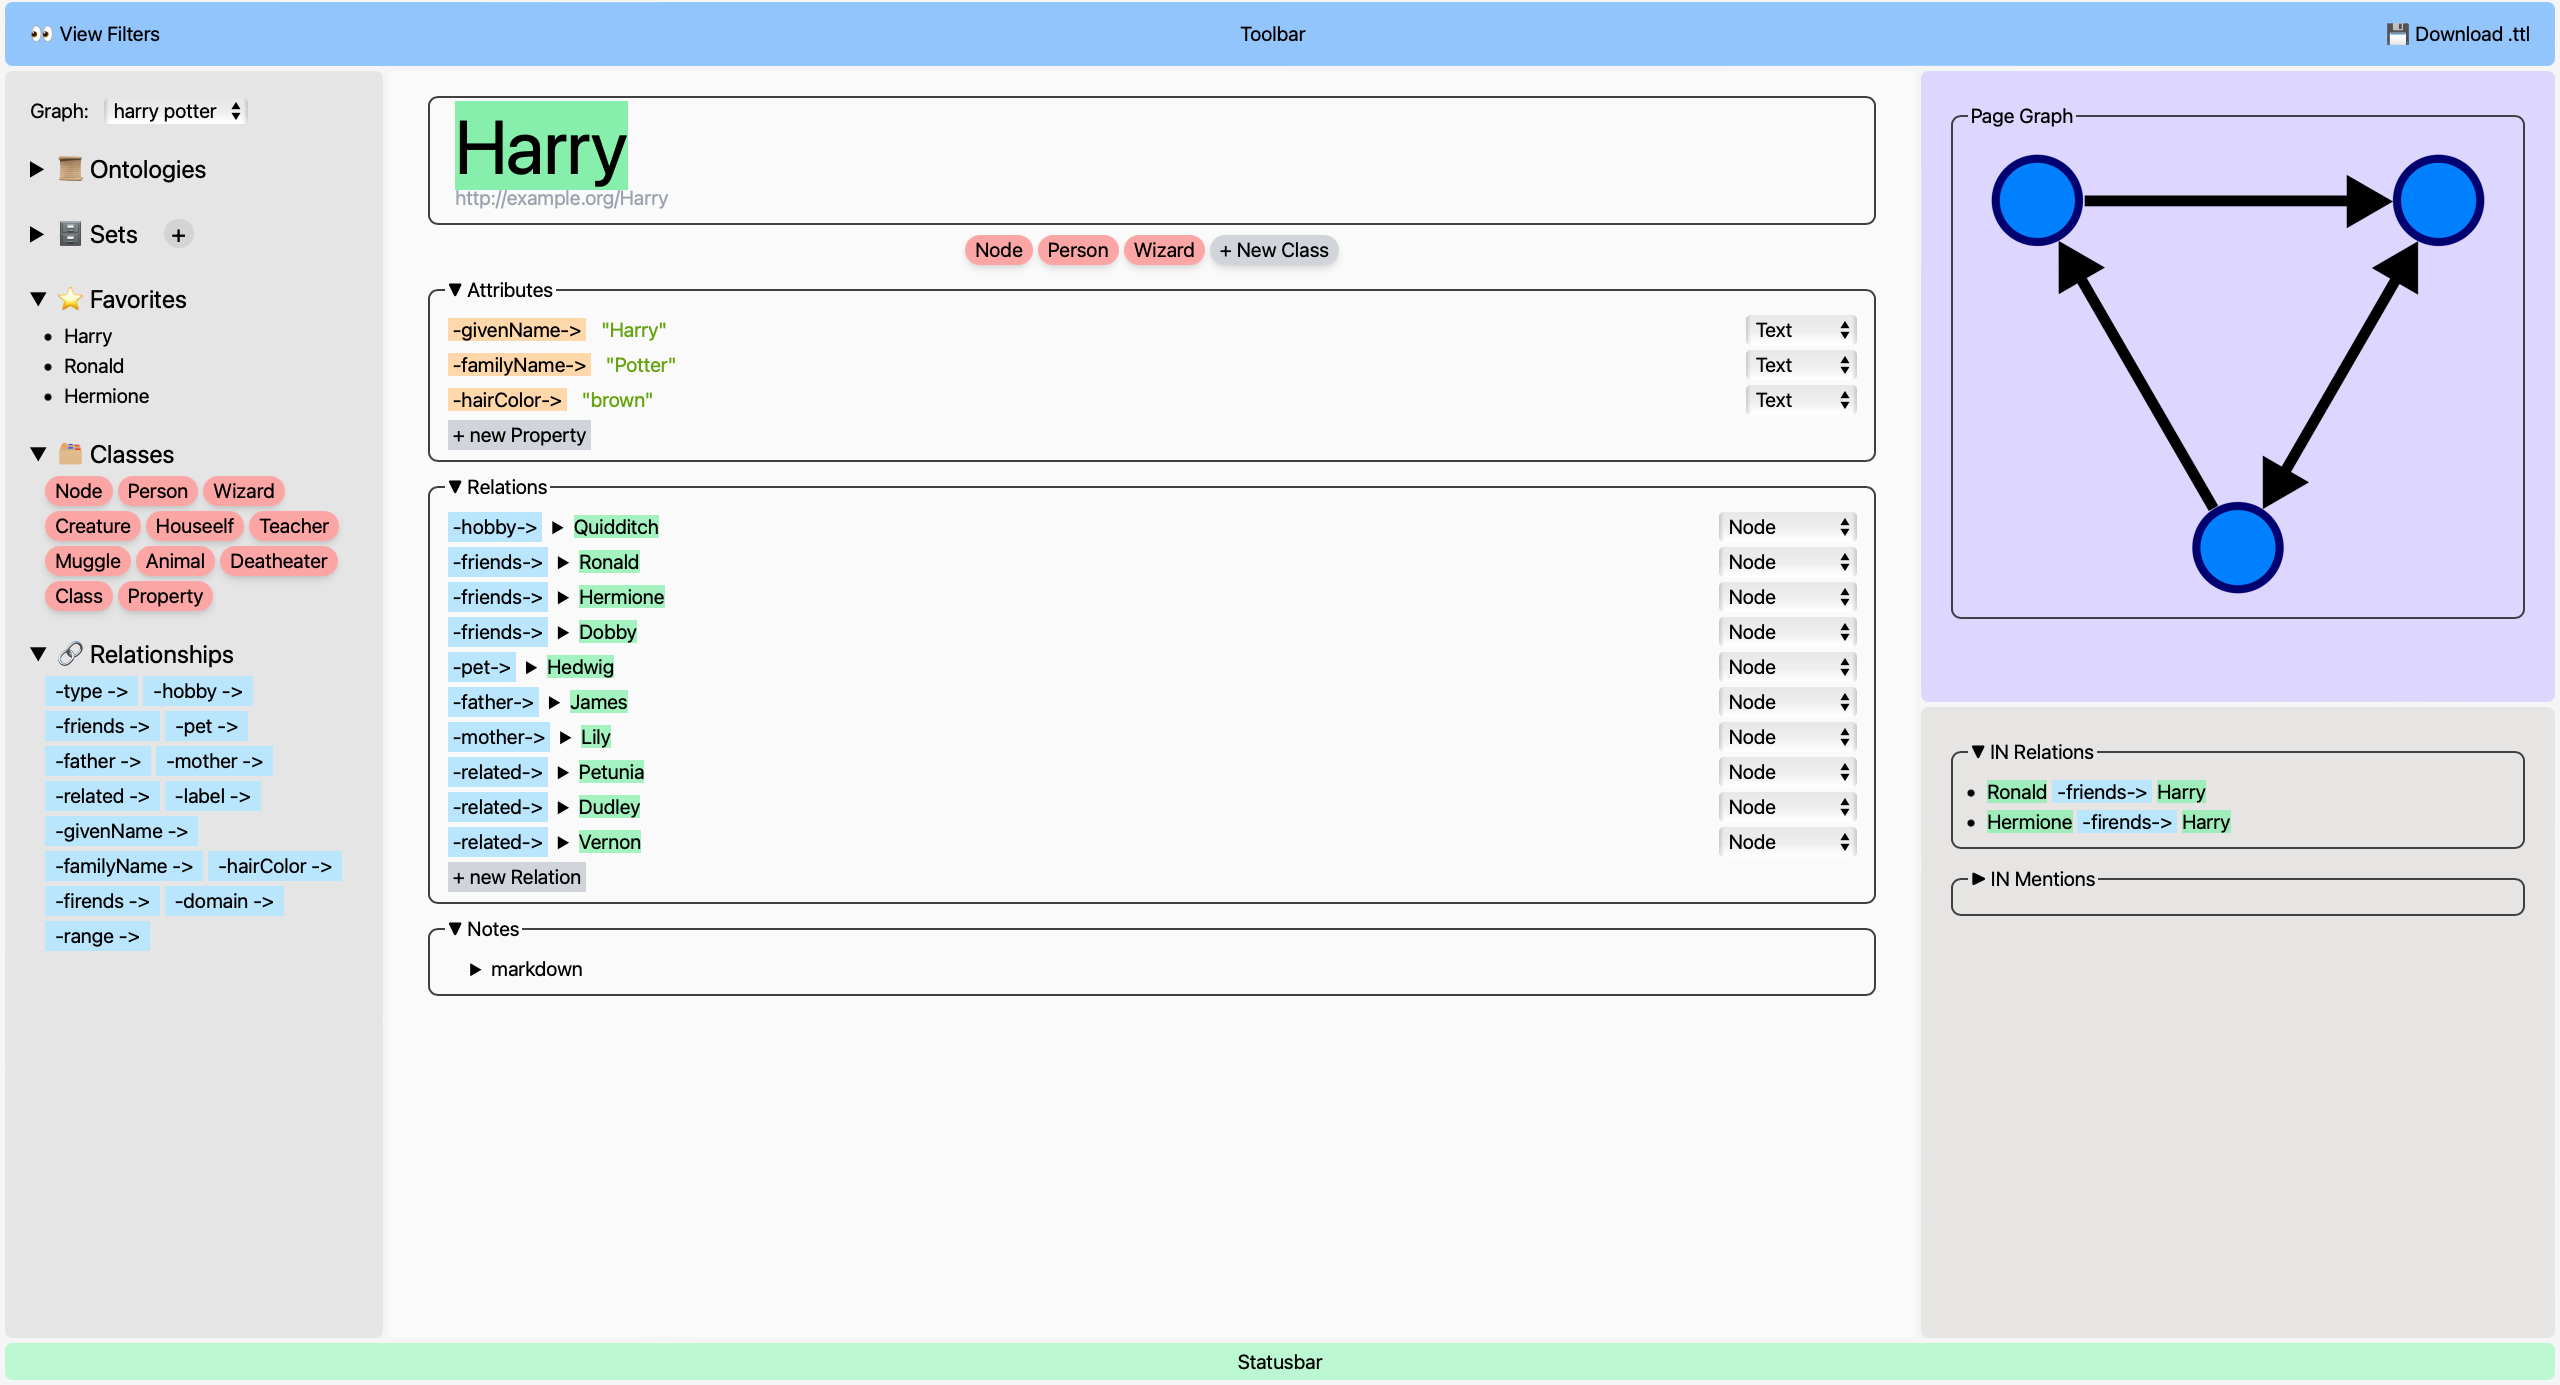
\includegraphics[width=\textwidth]{nink}
    \caption[short cap]{long caption}
\end{figure}
\section{Requirements for a PKG App Ecosystem}
- memex 60 years later **must have** functionality
- and everything from yourself
\section{Analysis of the Software Landscape}
- include current State of PKM
- web app, to reduce UX friction of install, login etc
- reference to other PKB Tools
- what basic features are needed?
    - bi-links
    - sets
    - overview of
        - in/out arcs
        - in/out mentions
- what are advanced features the model is capable of and could be explored?
- even though a prototype was implemented on SWS compatible Graph structure, that was more to showcase how easily implemented these features are on a real graph structure, and to show hard to understand SWS Concepts can be abstracted away.

Include all algorithms from code? how things are inserted into triple store etc?

- required structure of Data:
    - define what a Node is (Class Node?)
    - define what a Title is (Literal Label?)
\section{Applying the Model}
\section{Abstracting away Technical Details of Semantic Web Technologies}
\section{Testing Usability}


\section{unsorted}
current note taking tools only save “snapshots” of files in themselves, while we need the actual files (audio, video, pdf, text etc) to be workable and openable in any program. pkg needs to be a file system / cloud drive

Knowledge Graph Summarization: store only what’s relevant to the user

Premise Pkg stored in a cloud. Like social media posts or cloud drives, set visibility in the graph

integration of external knowledge by clicking add node / triple on external RDF data

**Abstract 0.1**

Semantic Web Technologies have been slow to adopt / gain traction outside of the academic areas. While there are relevant use cases in the industry, they are living a nieche dasein and are a tough sell. the lack of education and accessible tools for SWT means these technologies don’t get the spread necessary to really be usable and enable a semantic Web experience. This leads to SWT being sparely used on the internet, with the userbase being mostly academics, and sparcely in the industry.

This paper presents the implementation of a tool that tackles the problem of making a Tool (Broser Extension) that makes SWT approachable to the layman internet user. The hope is, that such a tool can drive adoption through implementation in Browsers, creating awareness of the technology and it’s benefits for regular people and the industry.

To be able to reach laymans, the software needs to have exceptionally easy UX and availability.

This means:

- no installation process
- no required configuration / setup
- no prior knowledge about the technologys and terms involved

To achieve these goals, the optimal case would be for Semantic Web Technologies to be integrated into browsers as a feature. Just like users are able to interact with websites now, in the future they should be able to browse and enrich / extend the semantic web.

Semantic Web Technologies, should be embedded into browsers, the same as features like having tabs, creating bookmarks, password managers or having a history visualization.

we will explore the matured state of these ideas due to evolution through time, as well as through the removal of technical hurdles.

We are building a web app, for usability sake, but also because semantic web is about WEB

When **loading RDF into a human readable editor, you get a load of machine relevant meta crap**

- Knowledge Graph Summarization: store only what’s relevant to the user


\chapter{Discussion}

- people have been struggling to develop better mediums than text, for mainly x reasons:
    - people learn to read and write in school, they don’t learn information science or databases
    - 

\section{How will the tool be used by real users?}

\section{The Missing Global Ontoloty standard for Personal Knowledge}

\section{Why Graphs for personal Knowledge Bases?}

comparison of Text Documents / PDFs / Books to the Graph structure (hierarchy, chronology, sense of orientation / navigation)

- Use Cases of KG
    - Open
    - Enterprise
    - Personal
    - Collaborative PKGs?
\chapter{Conclusions}

%%%%%%%%%%%%%%%%%%%%%%%%%%%%%%%%%%%%%%%%%%%
% Appendices
%%%%%%%%%%%%%%%%%%%%%%%%%%%%%%%%%%%%%%%%%%%
% \appendix
% \input{appendices/equations.tex}
% \input{appendices/sessionprotocol.tex}
% \input{appendices/code.tex}

%%%%%%%%%%%%%%%%%%%%%%%%%%%%%%%%%%%%%%%%%%%
% Bibliography
%%%%%%%%%%%%%%%%%%%%%%%%%%%%%%%%%%%%%%%%%%%
\bibliographystyle{ieeetr}
\bibliography{references}

\end{document}